\documentclass[a4paper,12pt,twoside]{book}
\usepackage[brazil]{babel}
\usepackage[utf8]{inputenc}
\usepackage{amssymb}
\usepackage{enumerate}
\usepackage{tabulary}
\tymin=0.22\textwidth
\tymax=0.42\textwidth

%\usepackage[framemethod=TikZ]{mdframed}
\usepackage{tcolorbox}
\tcbuselibrary{breakable}
\tcbuselibrary{theorems}
%\usepackage{lipsum}

\usepackage{fullpage}

\newtcbtheorem{professor}{Para o Professor}%
{colback=purple!15,colframe=purple,fonttitle=\bfseries}{th}
\newtcbtheorem{introdutorio}{Introdutório}%
{colback=green!5,colframe=green!35!black,fonttitle=\bfseries}{th}
\newtcbtheorem{abstrato}{Modelo abstrato}%
{colback=green!5,colframe=green!35!black,fonttitle=\bfseries}{th}
\newtcbtheorem{conexoes}{Conexões}%
{colback=green!5,colframe=green!35!black,fonttitle=\bfseries}{th}
\newtcbtheorem{explorando}{Explorando}%
{colback=green!5,colframe=green!35!black,fonttitle=\bfseries}{th}
\newtcbtheorem{massa}{Mão na massa}%
{colback=green!5,colframe=green!35!black,fonttitle=\bfseries}{th}
\newtcbtheorem{exercicio}{Exercício}%
{colback=gray!15,colframe=gray,fonttitle=\bfseries}{th}
\newtcbtheorem{resposta}{Resposta}%
{colback=blue!5,colframe=blue,fonttitle=\bfseries}{th}
\newtcbtheorem{imagem}{Imagem}%
{colback=yellow!15,colframe=yellow,fonttitle=\bfseries}{th}
\newtcbtheorem{figura}{Figura}%
{colback=green!5,colframe=green!35!black,fonttitle=\bfseries}{th}
\newtcbtheorem{nota}{Nota}%
{colback=gray!5,colframe=gray!35!black,fonttitle=\bfseries}{th}

\begin{document}

\chapter{ LIÇÃO 1 - Começando a falar sobre frações }


\includegraphics[width=\textwidth,height=4cm, keepaspectratio]{/var/www/livro/data/gitrepo/media/anchor/prologo}



\begin{professor*}[breakable]{}{}   Esta lição tem por objetivo introduzir frações unitárias a partir de modelos visuais contínuos, tais como   ``discos''  ,   ``retângulos''  ,   ``hexágonos''   e   ``segmentos''  , fazendo uso de expressões verbais como, por exemplo,   ``metade de...''  ,   ``um terço de...''  ,   ``a terça parte de...''  ,   ``um quarto de...''  , para indicar essas frações.    
  
  As atividades visam à observação da partição de uma unidade. O objetivo é levar o aluno a reconhecer diferentes modos de dividir e recompor a unidade. Não se pretende apresentar aos alunos a linguagem simbólica de fração unitária, que será tratada nos capítulos seguintes. Espera-se que, ao final da lição, os alunos saibam identificar e representar frações unitárias a partir de modelos visuais diversos, fazendo o uso adequado de expressões verbais para nomeá-las. No entanto, o professor não deve apresentar o termo   ``fração unitária''   ao estudante, uma vez que é desnecessário para a aprendizagem pretendida para o conceito. Fazê-lo pode, inclusive, afastar o foco que pretende-se na lição.  
  
  De maneira geral, as atividades envolvem a abordagem das frações unitárias em contextos diversos. Por exemplo, para diferenciar a divisão da unidade em partes   ``quaisquer''   da divisão da unidade em partes   ``iguais''   (equipartição); para reconhecer a necessidade de uma expressão verbal que identifique uma das partes iguais em uma equipartição da unidade; para perceber que a unidade pode ser subdividida em uma quantidade igual de partes sem que essa divisão represente uma equipartição; para reconhecer que, em uma equipartição, as partes podem não ter a mesma forma; para distinguir uma equipartição específica dentre partições diversas ou para reconhecer a quarta parte como a metade da metade.  
  
  A participação do aluno, criando representações próprias e fazendo o uso da linguagem verbal para explicar o seu raciocínio diante da realização das atividades, será fundamental na condução desta seção.  
  
  OBJETIVOS ESPECÍFICOS DA LIÇÃO 1:  
  O aluno deve ser capaz de:  
\begin{itemize} %s
    \item       Diferenciar uma partição qualquer de uma equipartição (partição em partes iguais) de um mesmo objeto e identificar a fração unitária correspondente.
    \item       Identificar, a partir de representações visuais diversas, frações unitárias de denominador variando de 2 a 10. 
    \item       Utilizar a linguagem verbal que caracteriza as frações unitárias de denominador variando de 2 a 10. (Isto é,       ``metade de''      ,       ``um meio''      ,       ``um terço''      ,       ``terça parte de''      , ...       ``um décimo''      ,       ``décima parte de''      ).
    \item       Comparar frações unitárias em exemplos concretos simples (Por exemplo, reconhecer que um terço de uma pizza é maior do que um quarto da mesma pizza).
    \item       Recompor a unidade a partir de uma fração unitária dada em modelos contínuos. 
    \item       Relacionar uma fração da unidade à quantidade necessária dessas partes para compor a unidade. Assim, por exemplo, é necessário reunir cinco       {\it quintas partes}       para recompor o todo.  
\end{itemize} %s
  
\end{professor*}






\chapter{ EXPLORANDO O ASSUNTO }


\includegraphics[width=\textwidth,height=4cm, keepaspectratio]{/var/www/livro/data/gitrepo/media/anchor/ativ_equiparticao}
\section{Atividade}




\begin{professor*}[breakable]{}{}   Objetivos específicos: Levar o aluno a   
\begin{itemize} %s
    \item       Diferenciar a divisão da unidade em partes       ``quaisquer''       da divisão da unidade em partes       ``iguais''       (equipartição). 
    \item       Reconhecer a necessidade de uma expressão verbal que identifique uma das partes iguais em uma equipartição da unidade.
    \item       Diferenciar       ``a divisão da unidade em três partes quaisquer''       da       ``divisão da unidade em três partes iguais''      . 
    \item       Compreender as expressões       ``um terço de''       e       ``terça parte de''       como forma de identicar uma das partes da equipartição da unidade em três partes. 
\end{itemize} %s
  
  
  
  
  Recomendações e sugestões para o desenvolvimento da atividade:  
\begin{itemize} %s
    \item       Recomenda-se que a atividade seja desenvolvida em grupos de 3 a 5 alunos. 
    \item       Busque conduzir a discussão nos grupos de modo que os estudantes percebam que, para que os irmãos recebam a mesma quantidade de chocolate, a divisão proposta para a barra de chocolate deve ser em       ``partes iguais''      , no sentido de ganharem todos a mesma quantidade de chocolate, não necessariamente pedaços de mesma forma.
    \item       Na discussão, procure destacar que a referência à       ``divisão em três partes iguais''       se dá (igualmente) a partir das expressões       ``um terço''       da barra de chocolate ou       ``a terça parte''       da barra de chocolate.
    \item       O item (d), provavelmente, pode não ser respondido corretamente pelos alunos. Se for o caso, as expressões       ``um terço de''       e       ``a terça parte de''       devem ser apresentadas. 
    \item       Fique atento às falas dos alunos. Observe que os alunos podem representar e verbalizar as respostas de diferentes modos e que não há uma resposta única para a atividade. Por exemplo, alguns alunos podem precisar de mais tempo do que outros para usar a expressão       ``um terço''       no lugar de       ``divisão em três partes iguais''      . Ou ainda, observarem que há diferentes representações para a equipartição. Por exemplo, 
\end{itemize} %s
  
  
  \begin{imagem*}[breakable]{}{}    
    PÁGINA DE REPRODUÇÃO    
    
    - FIGURA ARTÍSTICA -    
    
    Imagens: a mesma barra de chocolate que aparece na figura correspondente à atividade, divida exatamente como na imagem (instrução a seguir), e as partes separadas para serem reproduzidas isoladamente (como no exemplo).    
    
        \includegraphics[width=120pt, keepaspectratio]{/var/www/livro/data/gitrepo/media//cap1/secoes/chocolate_2.jpg}          
    
        \includegraphics[width=120pt, keepaspectratio]{/var/www/livro/data/gitrepo/media//cap1/secoes/chocolate_3.jpg}    
  \end{imagem*}  
  
\begin{itemize} %s
    \item       Esta atividade pode ser adaptada para alunos com deficiência de visão. Para isso, sugere-se confeccionar os modelos da barra de chocolate  inteira e repartida, que estão disponíveis para reprodução (      {\bf Inserir LINK de página para reprodução}      ), em três materiais diferentes. Por exemplo, papel comum e papéis com texturas diferentes, tecido ou material emborrachado.  
\end{itemize} %s
  
  
\end{professor*}


Três irmãos vão repartir uma barra de chocolate. Um deles sugere a seguinte divisão: 

\begin{imagem*}[breakable]{}{}   - FIGURA ARTÍSTICA   
  
  Na imagem devem estar 3 irmãos, aparentando idades diferentes (um deles pode ser cadeirante, por exemplo), observando uma única barra de chocolate retangular (preferencialemnte, imagem tridimensional sem subdivisões) repartida em três partes com tamanhos diferentes. Por exemplo:  
  
    \includegraphics[width=180pt, keepaspectratio]{/var/www/livro/data/gitrepo/media/cap1/secoes/licao1_1.png}  
  
\end{imagem*}

\begin{enumerate} [\quad a)] %d
  \item     Você concorda com essa divisão? Explique.
  \item     Com essa divisão, os três irmãos receberão a mesma quantidade de chocolate?
  \item     Use a imagem a seguir para mostrar uma divisão da barra de chocolate que permita que os 3 irmãos recebam quantidades iguais de chocolate. 
\end{enumerate} %d
\begin{imagem*}[breakable]{}{}    - FIGURA ARTÍSTICA - Inserir imagem da mesma barra retangular de chocolate da ilustração anterior sem qualquer partição sugerida. Apenas a imagem da barra de chocolate. Não há necessidade de ilustrar os irmãos.\end{imagem*}
\begin{enumerate} [\quad a)] %d
  \item     Considerando a divisão da barra de chocolate em 3 partes iguais, como você nomearia a quantidade de chocolate que cada irmão receberia? 
\end{enumerate} %d



\begin{resposta*}[breakable]{}{}  
\begin{enumerate} [\quad a)] %d
    \item       Este item não possui resposta correta, apenas respostas coerentes com a explicação do aluno. Por exemplo, um estudante pode dizer que sim e explicar que o irmão mais velho deve ficar com uma parte maior porque precisa de mais energia. Mas a resposta esperada é que a divisão não é justa porque as quantidades de chocolate são diferentes.
    \item       Não, eles receberão quantidades diferentes de chocolate, embora cada um receba um único pedaço do chocolate.
    \item       Respostas possíveis:
\end{enumerate} %d
  \begin{imagem*}[breakable]{}{}      - FIGURA ARTÍSTICA -    \mbox{} \newline              \includegraphics[width=360pt, keepaspectratio]{/var/www/livro/data/gitrepo/media/cap1/secoes/licao1_atv1.png}    \mbox{} \newline      ilustração: Cambrainha   \end{imagem*}  
\begin{enumerate} [\quad a)] %d
    \item       Cada parte é       ``um terço''       da barra ou a       ``terça parte''       da barra.
\end{enumerate} %d
  
\end{resposta*}





\includegraphics[width=\textwidth,height=4cm, keepaspectratio]{/var/www/livro/data/gitrepo/media/anchor/ativ_equiparticao2}
\section{Atividade}




\begin{professor*}[breakable]{}{}  
  
  Objetivos específicos: Levar o aluno a  
  
\begin{itemize} %s
    \item       Perceber que a unidade (no caso, uma pizza) pode ser subdividida em uma quantidade igual de partes sem que essa divisão represente uma equipartição.
    \item       Distinguir uma equipartição dentre partições diversas.
    \item       Diferenciar       ``a divisão da unidade em quatro partes quaisquer''       da       ``divisão da unidade em quatro partes iguais''      . 
    \item       Compreender as expressões       ``um quarto de''       e       ``quarta parte de''       como forma de identicar uma das partes da equipartição em 4 partes. 
\end{itemize} %s
  
  
  Recomendações e sugestões para o desenvolvimento da atividade:  
     
\begin{itemize} %s
    \item       Recomenda-se que a atividade seja desenvolvida em grupos de 3 a 5 alunos.
    \item       As diversas soluções apresentadas pelos diferentes grupos devem ser discutidas com a turma inteira. 
    \item       É possível que os alunos utilizem expressões variadas para nomear as partes de pizzas em cada divisão. Por exemplo,       ``a maior quarta parte''      ,       ``a menor quarta parte''      ,       ``as quartas partes iguais entre si''      ,       ``a menor parte''      ,       ``a maior parte''      , dentre outras. É importante que a discussão conduza os alunos ao entendimento de que apenas as partes da equipartição podem ser chamadas de       ``quartos''       da pizza, as demais são simplesmente fatias ou pedaços, por exemplo. 
    \item       Os alunos devem reconhecer que apenas uma das repartições propostas sugere a equipartição, respondendo assim, a última questão proposta nesta atividade.
    \item       Na ilustração, as crianças dos grupos em que a pizza não possui fatias com iguais quantidades de pizza parecem contrariadas. Recomenda-se levantar a questão:       ``por que será que elas estão parecendo zangadas?''
    \item       Essa atividade pode ser adaptada para alunos com deficiência visual. Para isso, sugere-se confeccionar os modelos das três pizzas repartidas, que estão disponíveis para reprodução (      {\bf Inserir LINK de página para reprodução}      ), em três materiais diferentes. Por exemplo, papel comum e papéis com texturas diferentes, tecido ou material emborrachado. 
\end{itemize} %s
  
  
  \begin{imagem*}[breakable]{}{}      - FIGURA ARTÍSTICA     
    \begin{nota*}[breakable]{}{}       NA PÁGINA PARA REPRODUCAO - INCLUIR a imagem das 3 pizzas repartidas: inteiras e com as respectivas partes isoladas.      
    \end{nota*}    
    
        \includegraphics[width=300pt, keepaspectratio]{/var/www/livro/data/gitrepo/media/cap1/secoes/licao1_atv2.png}    
    ilustração: Cambrainha    
    
  \end{imagem*}  
\end{professor*}


Três pizzas inteiras, de mesmo tamanho, foram repartidas entre as crianças de uma turma. Para isso, a turma foi dividida em três grupos com quatro crianças cada. Veja como cada grupo repartiu a sua pizza.

\begin{imagem*}[breakable]{}{}    - FIGURA ARTÍSTICA - A imagem deve conter 3 GRUPOS com 4 CRIANÇAS cada (Diversificar as características físicas das crianças). Cada um dos grupos deve estar observando uma pizza. Colocar duas das crianças do grupo 3 com feições   ``contrariadas''  . As pizzas devem ter mesmos tamanho e formato. As pizzas devem estar repartidas de três maneiras diferentes, como indicado nas imagens a seguir: Grupo 1, Grupo 2 e Grupo 3:   
  
    \includegraphics[width=300pt, keepaspectratio]{/var/www/livro/data/gitrepo/media/cap1/secoes/licao1_atv2.png}  
  
  ilustração: Cambrainha  
  
\end{imagem*}

\begin{enumerate} [\quad a)] %d
  \item     Cada um dos três grupos repartiu a sua pizza na mesma quantidade de fatias que os outros grupos?
  \item     Dessa maneira, todas as crianças da turma receberam a mesma quantidade de pizza?
  \item     Em algum dos grupos as 4 crianças receberam a mesma quantidade de pizza? Se sim, em qual? Considerando a pizza inteira, como você nomearia cada uma das fatias de pizza desse grupo? 
\end{enumerate} %d



\begin{resposta*}[breakable]{}{}  
\begin{enumerate} [\quad a)] %d
    \item       Sim. Cada grupo repartiu sua pizza em quatro fatias.
    \item       Não, pois algumas fatias têm quantidades de pizza diferentes das outras.
    \item       Apenas no grupo 1 as 4 crianças receberam a mesma quantidade de pizza. Cada fatia da pizza do grupo 1 é       ``um quarto''       da pizza ou       ``a quarta parte''       da pizza. Diferentemente das demais pizzas.
\end{enumerate} %d
  
\end{resposta*}



\includegraphics[width=\textwidth,height=4cm, keepaspectratio]{/var/www/livro/data/gitrepo/media/anchor/ativ_enfeite}
\section{Atividade}




\begin{professor*}[breakable]{}{}  
  Objetivo específico:  
\begin{itemize} %s
    \item       Abordar a equipartição em um modelo linear.
    \item       Reconhecer a quarta parte como a metade da metade.
\end{itemize} %s
  
  
  Recomendações e sugestões para o desenvolvimento da atividade:  
  
\begin{itemize} %s
    \item       Recomenda-se que esta atividade seja desenvolvida em grupos de quatro alunos. 
    \item       Cada grupo deve receber um pedaço de barbante de, aproximadamente, 1m e quatro enfeites (todos iguais).  
    \item       Os quatro enfeites precisam ser confeccionados antes da realização da tarefa. Sugerem-se estrelas, cujos modelos estão disponíveis para reprodução       {\bf (Inserir LINK de página para reprodução)}      . No entanto, segundo a avaliação do professor, os enfeites podem ser outros, desde que sejam os 4 congruentes.
    \item       Como sugestão, se possível, solicitar aos alunos que confeccionem os enfeites, por exemplo, associando esta atividade com geometria, com a abordagem de grandezas e medidas, com a disciplina de artes ou envolvendo culturas artesanais populares.
    \item       A equipartição do barbante não deve ser obtida a partir da medida do barbante, mas por sucessivas dobras do barbante sobre ele mesmo, como ilustrado na resposta da atividade.
    \item       A manipulação e a dobra do barbante devem sustentar a discussão para a identificação da       ``metade da metade''       com a       ``quarta parte''       do barbante. Nesse caso, a identificação se dará pela sobreposição das partes. 
\end{itemize} %s
  
\end{professor*}


Alice quer enfeitar a sala de aula e pretende prender os enfeites utilizando pedaços de barbante. Para isso, quer cortar o barbante em pedaços iguais, para que os enfeites fiquem todos da mesma altura. Ajude Alice a cortar o barbante.

\begin{imagem*}[breakable]{}{}    - FIGURA ARTÍSTICA - Incluir imagem de um pedaço de barbante e de 4 estrelas congruentes, como ilustrado a seguir:  
  Alice é uma menina morena de rabo de cavalo. Ela será um personagem frequente deste livro.  
  
    \includegraphics[width=180pt, keepaspectratio]{/var/www/livro/data/gitrepo/media//cap1/secoes/alice_barbante_estrelas.jpg}  
\end{imagem*}

\begin{imagem*}[breakable]{}{}   - FIGURA ARTÍSTICA -  
  \begin{nota*}[breakable]{}{}         
    INCLUIR PÁGINA DE REPRODUÇÃO COM apenas 1 ESTRELA com aproximadamente 10 cm de altura para ser recortada.    
  \end{nota*}  
\end{imagem*}


\begin{resposta*}[breakable]{}{}   Uma maneira de se cortar o barbante é dobrar ao meio e depois dobrar novamente ao meio obtendo quatro partes iguais como ilustrado na figura a seguir.  
  \begin{imagem*}[breakable]{}{}     - FIGURA ARTÍSTICA - Sequência de duas imagens que ilustrem um barbante sendo dobrado sobre ele mesmo duas vezes sucessivas, até que se obtenha quartos. Por exemplo, como a imagem a seguir:    
        \includegraphics[width=180pt, keepaspectratio]{/var/www/livro/data/gitrepo/media//cap1/secoes/barbante_dobras.jpg}    
  \end{imagem*}  
\end{resposta*}



\includegraphics[width=\textwidth,height=4cm, keepaspectratio]{/var/www/livro/data/gitrepo/media/anchor/conexoes}

\chapter{ ORGANIZANDO AS IDEIAS }


\begin{professor*}[breakable]{}{}     
  
  Nesta etapa, não se espera que os alunos compreendam as frações como números. O objetivo é que percebam seu papel para expressar quantidades em situações de equipartição da unidade. Assim, as frações podem ser utilizadas no dia a dia para identificar quantidades do mesmo modo que os números naturais, já conhecidos dos alunos. Por exemplo, como nas expressões:   ``dois ovos''  ,   ``duas xícaras de farinha''  ,   ``um terço de xícara de cacau''   e   ``meio litro de leite''  .  
  
  Objetiva-se a expressão verbal e não a representação simbólica. Espera-se, assim, que os alunos apropriem-se das expressões verbais que identificam as frações unitárias (um meio, um terço, um quarto, ... , um nono e um décimo, antes de serem apresentados formalmente à simbologia matemática (que será objetivo da próxima lição).  A referência às frações unitárias com a expressão   ``um''   antes da identicação da parte, como, por exemplo, em   ``um terço''   e em   ``um sétimo''   é uma decisão pedagógica. Claro que é possível se referir a essas frações  simplesmente por   ``terço''   e   ``sétimo''  , respectivamente. No entanto, nas próximas seções, pretende-se que as frações não unitárias, como   ``dois terços''   e   ``nove sétimos''  , por exemplo, sejam entendidas a partir da justaposição das frações unitárias correspondentes, o que é naturalmente amparado pela contagem. Nas expressões verbais relativas às frações unitárias, o   ``um''   antes da identificação da parte está associado à cotagem. Dessa formma, a compreensão das frações   ``um terço''   e   ``dois terços''   ou das frações   ``um sétimo''   e   ``nove sétimos''  , por exemplo, seguem a mesma construção lógica.    
  
\end{professor*}  


Os números que você havia estudado até aqui são usados para contar, ordenar e rotular, e são chamados números naturais.
\begin{imagem*}[breakable]{}{}   - FIGURA ARTÍSTICA - ESTA IMAGEM PRECISA SER REFEITA.  
    \includegraphics[width=360pt, keepaspectratio]{/var/www/livro/data/gitrepo/media//cap1/secoes/numeros-naturais-01.png}  
\end{imagem*}

Para que servem os números naturais?

As atividades que foram apresentadas nesta lição lidam com quantidades não inteiras: um terço de uma barra de chocolate, um quarto de pizza, por exemplo. 
Outros exemplos aparecem no nosso dia a dia: ``o ser humano passa um terço de sua vida dormindo'', ``eu tomei a metade de um copo de leite''. 
Nas atividades que realizamos, uma barra de chocolate, pizzas e um pedaço de barbante foram repartidos em partes iguais. 
Nesses casos, a barra de chocolate, uma pizza e o pedaço de barbante são vistos como unidades. 
Cada uma das partes em que essas unidades foram repartidas igualmente é uma fração da unidade.

\begin{imagem*}[breakable]{}{}   - FIGURA ARTÍSTICA -  
  {\bf Imagem de uma pizza e de um pedaço de barbante, cada um dividido em 4 partes.}  
\end{imagem*}

O nome dado à fração da unidade depende da quantidade de partes em que a unidade é dividida. 

Ao dividir uma unidade qualquer em duas partes iguais ou ao meio, cada uma das partes é chamada de {\it um meio} ou {\it a metade} da unidade. 

Por exemplo, se uma barra de chocolate é repartida igualmente entre dois amigos, a quantidade que caberá a cada um dos amigos é {\it um meio} da barra de chocolate (ou {\it metade} da barra). Nesse exemplo, a unidade é a barra de chocolate.

\begin{imagem*}[breakable]{}{}   - FIGURA ARTÍSTICA - INCLUIR IMAGENS ILUSTRATIVA de metade   
  {\bf Imagem de duas crianças a barra de chocolate em que a metade é identificada}  
\end{imagem*}

Ao dividir uma unidade em três partes iguais, cada uma das partes é chamada de {\it um terço} ou {\it a terça parte} da unidade. 

Por exemplo, se, em uma receita de bolo, é necessário acrescentar {\it um terço} de um litro de leite. Isso significa que, para colocar a quantidade correta de leite na receita, é preciso repartir o litro de leite em três partes iguais e usar apenas uma dessas partes, que é {\it um terço} do litro de leite. Nesse caso, a unidade é um litro de leite.

\begin{imagem*}[breakable]{}{}   - FIGURA ARTÍSTICA - INCLUIR IMAGEM ILUSTRATIVA de terço   
  {\bf Sobre uma mesa, uma garrafa cilindrica cheia de leite e três garrafas iguais ao lado, cada uma com 1/3 da capacidade prennchida.}  
  
  Por exemplo:   
    \includegraphics[width=60pt, keepaspectratio]{/var/www/livro/data/gitrepo/media//cap1/secoes/litro_de_leite.jpg}  
    \includegraphics[width=60pt, keepaspectratio]{/var/www/livro/data/gitrepo/media//cap1/secoes/um_terco_de_litro_de_leite.jpg}  
  
\end{imagem*}

Ao dividir uma unidade em quatro partes iguais, cada uma das partes é chamada de {\it um quarto} ou {\it quarta parte} da unidade. 

Por exemplo,
A parte colorida da figura é um quarto da figura. Neste caso, a figura é a unidade.


\begin{imagem*}[breakable]{}{}   - FIGURA ARTÍSTICA - INCLUIR IMAGEM ILUSTRATIVA de quartos  
    \includegraphics[width=120pt, keepaspectratio]{/var/www/livro/data/gitrepo/media//cap1/secoes/quartos_conexoes.jpg}  
   \end{imagem*}

Da mesma forma, ao dividir uma unidade em cinco partes iguais, cada uma das partes é chamada de {\it um quinto} ou {\it quinta parte} da unidade.

Por exemplo,
{\it um quinto} de todo ouro pesado nas Casas de Fundição no Brasil era pago em impostos à Coroa Portuguesa. Desta forma, a quantidade de ouro pago em impostos à Coroa Portuguesa era igual a {\it um quinto} ou a {\it quinta parte} do ouro pesado nas Casas de Fundição no Brasil.

\begin{imagem*}[breakable]{}{}   - FIGURA ARTÍSTICA - INCLUIR IMAGEM ILUSTRATIVA de quintos   
  {\bf Um homem entregando um saco de ouro a um rei e ficando com outros 4 sacos}  
\end{imagem*}









\chapter{ MÃO NA MASSA }


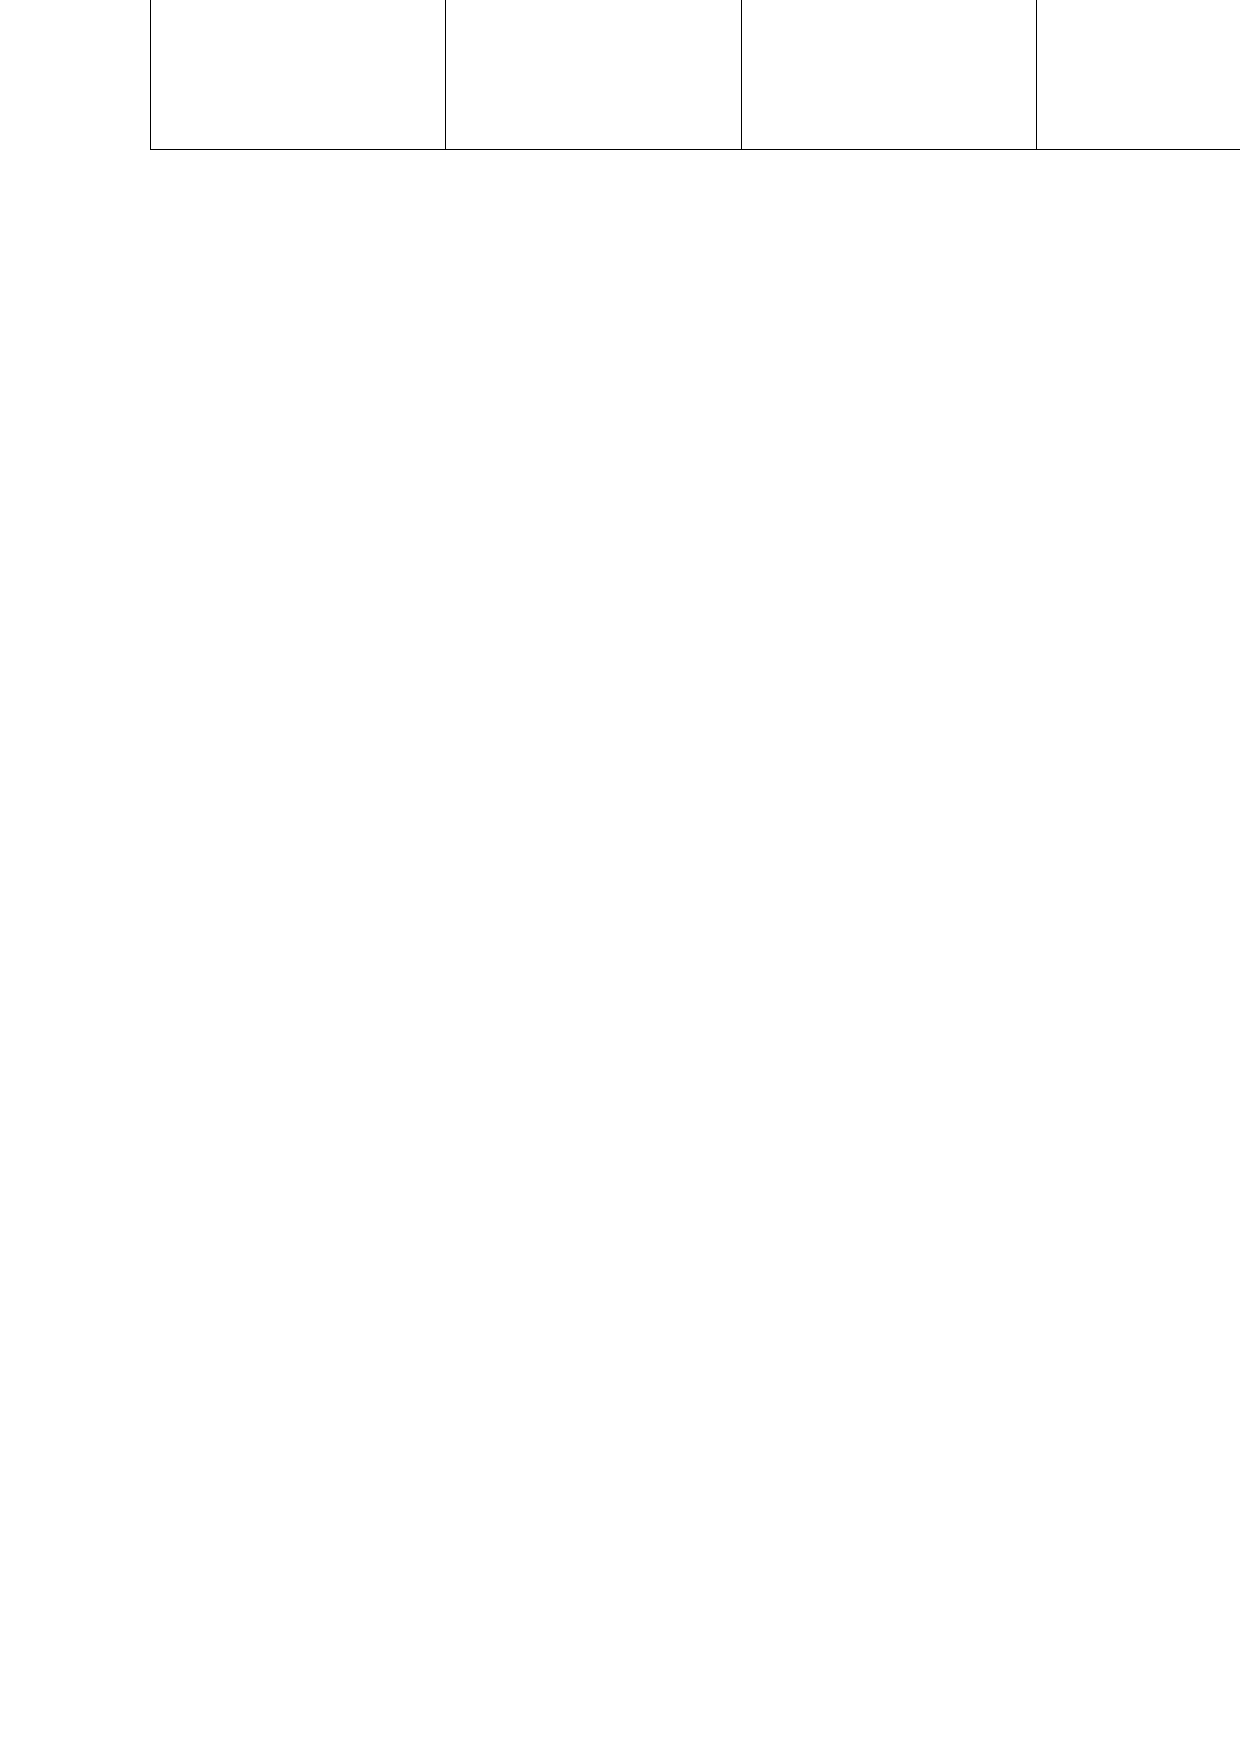
\includegraphics[width=\textwidth,height=4cm, keepaspectratio]{/var/www/livro/data/gitrepo/media/anchor/ativ_retangulos_coloridos}
\section{Atividade}




\begin{professor*}[breakable]{}{}     
  Objetivo específico: Levar o aluno a:  
\begin{itemize} %s
    \item       Reconhecer que, em uma equipartição, as partes podem não ter a mesma forma. 
    \item       Identificar a equivalência entre as partes de uma equipartição a partir de sobreposição ou da comparação pelo reconhecimento da associação a uma mesma fração unitária (no caso, 1/4).
    \item       Reconhecer a quarta parte como a metade da metade.
\end{itemize} %s
  
  
  Recomendações e sugestões para o desenvolvimento da atividade:  
  
\begin{itemize} %s
    \item       Recomenda-se que esta atividade seja desenvolvida em grupos de 3 a 5 alunos. Cada grupo deve receber as imagens dos oito retângulos, disponíveis para reprodução       {\bf (Inserir LINK de página para reprodução)}       e colorí-las, cada um com uma cor diferente das demais.
    \item       Em cada grupo, os alunos devem decidir qual (ou quais) das divisões propostas para os retângulos correspondem a uma partição em quartos. É importante observar que todos os retângulos estão divididos em quartos.
    \item       Conduza a discussão de modo a levar os alunos a reconhecer que, em uma equipartição, as partes não precisam ter a mesma forma.   
    \item       Se necessário, o professor pode associar cada retângulo a um objeto concreto (por exemplo, uma barra de chocolate ou a um pedaço de bolo). No entanto, nesta atividade, espera-se que os alunos consigam lidar com a figura de um retângulo como representativa de um todo genérico. 
    \item       Recomenda-se que os alunos recortem as partes de cada um dos retângulos para realizar a comparação por sobreposição. No entanto, essa estratégia não será suficiente para todos os 8 casos. Em alguns casos, a comparação se dará pela identificação da fração unitária correspondente a cada parte. Nesses casos, o aluno deve reconhecer que a quarta parte é equivalente à metade da metade. Por exemplo, como no caso seguir.
\end{itemize} %s
  
  
  \begin{imagem*}[breakable]{}{}     Incluir imagem como a exemplificada a seguir, inclusive com os comentários indicados    
        \includegraphics[width=120pt, keepaspectratio]{/var/www/livro/data/gitrepo/media//cap1/secoes/metade_da_metade.jpg}    
  \end{imagem*}  
  
\begin{itemize} %s
    \item       Segundo a avaliação do professor, a atividade pode ser realizada em duas etapas. Em um primeiro momento, os alunos recebem quatro das oito imagens, Página A, e realizam a atividade com essas imagens - cuja comparação se dá apenas pela sobreposição. Em seguida, recebem as outras quatro, para concluir a atividade. Para as figuras da Página B, será necessário reconhecer a quarta parte como a metade da metade. É importante que o professor, ao final das duas etapas, avalie as escolhas como um todo.
\end{itemize} %s
  
  
  \begin{imagem*}[breakable]{}{}    
    \begin{nota*}[breakable]{}{}       - FIGURA GEOMÉTRICA - PÁGINA PARA REPRODUÇÃO      
      os retângulos devem estar organizados em duas páginas conforme a ilustração.       
                   \includegraphics[width=120pt, keepaspectratio]{/var/www/livro/data/gitrepo/media//undefined/quartos_encarte_1.jpg}                     \includegraphics[width=120pt, keepaspectratio]{/var/www/livro/data/gitrepo/media//cap1/secoes/quartos_encarte_2.jpg}      
    \end{nota*}    
  \end{imagem*}  
  
\end{professor*}


Quais dos retângulos a seguir foram repartidos em {\it quartos}?

\begin{imagem*}[breakable]{}{}   - FIGURA GEOMÉTRICA - A imagem deve conter oito retângulos   {\bf congruentes}   coloridos, cada um com uma cor diferente das demais. Os retângulos devem estar divididos em partes conforme a imagem   
    \includegraphics[width=120pt, keepaspectratio]{/var/www/livro/data/gitrepo/media//cap1/secoes/quartos.jpg}  
  
\end{imagem*}




\begin{resposta*}[breakable]{}{}  
  Todos os retângulos estão divididos em quartos.   
\end{resposta*}





\includegraphics[width=\textwidth,height=4cm, keepaspectratio]{/var/www/livro/data/gitrepo/media/anchor/refl_retangulos_coloridos}



\begin{refletindo*}[breakable]{}{}  
  Quando se diz que uma unidade é repartida em meios, terços, quartos, quintos, etc., a unidade foi repartida em 2, 3, 4, 5, etc. partes de mesma quantidade.  
  Na atividade acima, se os retângulos representam bolos (ou barras de chocolate), as quatro partes em que foram divididos os retângulos possuem mesma quantidade de bolo (ou de chocolate).  
  Os retângulos foram divididos em quartos, embora as partes não possuam mesma forma.  
\end{refletindo*}


\includegraphics[width=\textwidth,height=4cm, keepaspectratio]{/var/www/livro/data/gitrepo/media/anchor/ativ_ident_terco}
\section{Atividade}




\begin{professor*}[breakable]{}{}     
  Objetivo específico: Levar o aluno a;  
  
\begin{itemize} %s
    \item       Identificar uma mesma fração unitária (no caso, a terça parte) em representações diversas, ou seja, em representações da unidade não necessariamente congruentes.
\end{itemize} %s
  
     
  
  Recomendações e sugestões para o desenvolvimento da atividade:  
\begin{itemize} %s
    \item       Recomenda-se que esta atividade seja desenvolvida em grupos de 3 a 5 alunos.
    \item       Durante a discussão, os alunos devem ser estimulados a explicar as suas escolhas. A discussão sobre os motivos da identificação, ou não, de cada uma das representações à terça parte do todo correspondente será fundamental para atingir o objetivo da atividade.
    \item       Os alunos devem reconhecer que, independente da unidade considerada, em uma equipartição em 3 partes, cada uma das partes é um terço (ou a terça parte) da unidade.
    \item       Aproveite as próprias palavras e os argumentos dos alunos para conduzi-los às conclusões esperadas.
    \item       Fique atento aos alunos que selecionarem as figuras que simplesmente possuem alguma associação com o número 3, não correspondendo a terços. Por exemplo, um aluno que associe a       {\bf Figura ZZ}       a terços pode ainda não ter compreendido a necessidade da equipartição para a identificaçào de um terço. Já o aluno que associa       {\bf Figura ZZ}       a terços pode estar simplesmente contando as partes em vermelho, sem que tenha reconhecido que a figura deveria estar dividida em 3 partes iguais e não em 5. 
\end{itemize} %s
  
\end{professor*}



Em cinco das figuras a seguir a parte em vermelho é um terço da figura. Identifique estas figuras.
\begin{imagem*}[breakable]{}{}   - FIGURA GEOMÉTRICA - Estas figuras devem ser produzidas individualmente, importante levar em conta a fração. Não se deve colocar os itens A), B), etc.  
    \includegraphics[width=300pt, keepaspectratio]{/var/www/livro/data/gitrepo/media//cap1/secoes/um_terco_vermelho.jpg}  
\end{imagem*}


\begin{resposta*}[breakable]{}{}  
  A parte em vermelho representa um terço da figura nos itens C), D), E), F) e H).   
\end{resposta*}




\includegraphics[width=\textwidth,height=4cm, keepaspectratio]{/var/www/livro/data/gitrepo/media/anchor/ativ_recomportodo}
\section{Atividade}




\begin{professor*}[breakable]{}{}  
  Objetivo específico: Levar o aluno a:  
\begin{itemize} %d
    \item       Recompor a unidade a partir de uma fração unitária dada em modelos contínuos. 
    \item       Relacionar uma fração da unidade à quantidade necessária dessas partes para compor a unidade. Assim, por exemplo, é necessário reunir cinco       {\it quintas partes}       para recompor o todo.
\end{itemize} %d
  
        
  
  Recomendações e sugestões para o desenvolvimento da atividade:  
\begin{itemize} %d
    \item       Recomenda-se que a atividade seja desenvolvida em grupos de 3 a 5 alunos.
    \item       É importante ter em mente que existem várias soluções para cada item. Por exemplo, o item 
\end{itemize} %d
    \includegraphics[width=18pt, keepaspectratio]{/var/www/livro/data/gitrepo/media/undefined/completar-o-todo-disco.jpg}   é metade de uma figura. Complete a figura para obter o todo. pode ser corretamente respondido por:     \includegraphics[width=36pt, keepaspectratio]{/var/www/livro/data/gitrepo/media/cap1/secoes/completar-o-todo-resposta-01.jpg}   ou     \includegraphics[width=36pt, keepaspectratio]{/var/www/livro/data/gitrepo/media/cap1/secoes/completar-o-todo-resposta-02.jpg}  .  
\begin{itemize} %d
    \item       Estimule os alunos a reconhecer (e a fazer) mais do que uma representação para o todo em cada item.
    \item       Estimule os alunos a, a partir da identificação da fração unitária, determinar a quantidade de partes necessárias para recompor o todo.
\end{itemize} %d
  
\end{professor*}


\begin{imagem*}[breakable]{}{}   FIGURAS GEOMÉTRICAS - As figuras das linhas devem ser feitas individualmente. Observe que há figuras no   ``Para o professor''   e na   ``Resposta''  .  
\end{imagem*}
\begin{enumerate} [\quad a)] %s
  \item     
\end{enumerate} %s
\includegraphics[width=18pt, keepaspectratio]{/var/www/livro/data/gitrepo/media/undefined/completar-o-todo-disco.jpg} é metade de uma figura. Complete a figura para obter a unidade.
\begin{enumerate} [\quad a)] %s
  \item     
\end{enumerate} %s
\includegraphics[width=18pt, keepaspectratio]{/var/www/livro/data/gitrepo/media/undefined/completar-o-todo-disco.jpg} é um terço de uma figura. Complete a figura para obter a unidade.
\begin{enumerate} [\quad a)] %s
  \item     
\end{enumerate} %s
\includegraphics[width=18pt, keepaspectratio]{/var/www/livro/data/gitrepo/media/undefined/completar-o-todo-disco.jpg} é um quarto de uma figura. Complete a figura para obter a unidade.
\begin{enumerate} [\quad a)] %s
  \item     
\end{enumerate} %s
\includegraphics[width=18pt, keepaspectratio]{/var/www/livro/data/gitrepo/media/undefined/completar-o-todo-quadrado.jpg} é metade de uma figura. Complete a figura para obter a unidade.
\begin{enumerate} [\quad a)] %s
  \item     
\end{enumerate} %s
\includegraphics[width=18pt, keepaspectratio]{/var/www/livro/data/gitrepo/media/undefined/completar-o-todo-quadrado.jpg} é um terço de uma figura. Complete a figura para obter a unidade.
\begin{enumerate} [\quad a)] %s
  \item     
\end{enumerate} %s
\includegraphics[width=18pt, keepaspectratio]{/var/www/livro/data/gitrepo/media/undefined/completar-o-todo-quadrado.jpg} é um quarto de uma figura. Complete a figura para obter a unidade.
\begin{enumerate} [\quad a)] %s
  \item     
\end{enumerate} %s
\includegraphics[width=18pt, keepaspectratio]{/var/www/livro/data/gitrepo/media/undefined/completar-o-todo-segmento.jpg} é metade de uma figura. Complete a figura para obter a unidade.
\begin{enumerate} [\quad a)] %s
  \item     
\end{enumerate} %s
\includegraphics[width=18pt, keepaspectratio]{/var/www/livro/data/gitrepo/media/undefined/completar-o-todo-segmento.jpg} é um terço de uma figura. Complete a figura para obter a unidade.
\begin{enumerate} [\quad a)] %s
  \item     
\end{enumerate} %s
\includegraphics[width=18pt, keepaspectratio]{/var/www/livro/data/gitrepo/media/undefined/completar-o-todo-segmento.jpg} é um quarto de uma figura. Complete a figura para obter a unidade.
\begin{enumerate} [\quad a)] %s
  \item     
\end{enumerate} %s
\includegraphics[width=24pt, keepaspectratio]{/var/www/livro/data/gitrepo/media/undefined/completar-o-todo-triangulo.jpg} é metade de uma figura. Complete a figura para obter a unidade.
\begin{enumerate} [\quad a)] %s
  \item     
\end{enumerate} %s
\includegraphics[width=24pt, keepaspectratio]{/var/www/livro/data/gitrepo/media/undefined/completar-o-todo-triangulo.jpg} é um terço de uma figura. Complete a figura para obter a unidade.
\begin{enumerate} [\quad a)] %s
  \item     
\end{enumerate} %s
\includegraphics[width=24pt, keepaspectratio]{/var/www/livro/data/gitrepo/media/undefined/completar-o-todo-triangulo.jpg} é um quarto de uma figura. Complete a figura para obter a unidade.


\begin{resposta*}[breakable]{}{}  
  Possibilidades de resposta  
  
    \includegraphics[width=360pt, keepaspectratio]{/var/www/livro/data/gitrepo/media/cap1/secoes/licao1_atv61_novo.png}  
  
  $\ $     
  
    \includegraphics[width=420pt, keepaspectratio]{/var/www/livro/data/gitrepo/media/cap1/secoes/licao1_atv6_2_novo.png}  
  
  ilustração:Cambrainha  
\end{resposta*}


\includegraphics[width=\textwidth,height=4cm, keepaspectratio]{/var/www/livro/data/gitrepo/media/anchor/ativ_desenhar}
\section{Atividade}




\begin{professor*}[breakable]{}{}  
  
  Objetivos específicos: Levar o aluno a:  
\begin{itemize} %s
    \item       Representar uma fração unitária a partir de uma unidade dada.  
    \item       Reconhecer (e obter) um quarto como a metade da metade e um oitavo como a metade de um quarto.
    \item       Comparar as frações unitárias metade, um quarto e um oitavo de um mesmo quadrado.
\end{itemize} %s
  
  
  Recomendações e sugestões para o desenvolvimento da atividade:  
\begin{itemize} %s
    \item       Essa é uma atividade que o aluno pode fazer individualmente. 
    \item       Não se espera que, nesta atividade, os alunos usem a medida para fazer a equipartição de maneira mais precisa. O objetivo é que fazer a equipartição livremente e de forma coerente. Assim, por exemplo, podem ser aceitas como respostas
\end{itemize} %s
  
  
    \includegraphics[width=90pt, keepaspectratio]{/var/www/livro/data/gitrepo/media/cap1/secoes/quadrado-resposta-01.png}   e     \includegraphics[width=90pt, keepaspectratio]{/var/www/livro/data/gitrepo/media/cap1/secoes/quadrado-resposta-02.png}  .  
  
  Já as representações a seguir sugerem que os alunos precisam revisar os conceitos exigidos para a solução da atividade:  
  
    \includegraphics[width=90pt, keepaspectratio]{/var/www/livro/data/gitrepo/media//cap1/secoes/quadrado-resposta-03.png}  
  
\begin{itemize} %s
    \item       A representação da unidade se dá de forma genérica por um quadrado. 
    \item       Espera-se que os alunos reconheçam que para obter um quarto pode determinar a metade da metade. E que, para obter um oitavo pode dividir um quarto ao meio.
    \item       Recomende que os alunos usem dobradura para identificar as frações pedidas.Assim, por exemplo, a fração       $\frac{1}{4}$       pode ser obtida por duas dobras do papel.    
    \item       Procure apresentar e discutir com a turma mais do que uma solução para cada item.
    \item       Discuta com os estudantes que quanto maior o número de partes iguais em que se particiona o quadrado, menor fica cada uma das partes.
\end{itemize} %s
  
\end{professor*}

\begin{imagem*}[breakable]{}{}   FIGURAS GEOMÉTRICAS - Observe que há figuras no   ``Para o professor''   e na   ``Resposta''  .  
\end{imagem*}

\begin{enumerate} [\quad a)] %d
  \item     Pinte metade do quadrado a seguir.
\end{enumerate} %d
\mbox{} \newline  \includegraphics[width=150pt, keepaspectratio]{/var/www/livro/data/gitrepo/media//cap1/secoes/um-meio-um-quarto-um-oitavo.jpg}
\begin{enumerate} [\quad a)] %d
  \item     Pinte um quarto do quadrado a seguir.
\end{enumerate} %d
\mbox{} \newline  \includegraphics[width=150pt, keepaspectratio]{/var/www/livro/data/gitrepo/media//cap1/secoes/um-meio-um-quarto-um-oitavo.jpg}
\begin{enumerate} [\quad a)] %d
  \item     Pinte um oitavo do quadrado a seguir.
\end{enumerate} %d
\mbox{} \newline  \includegraphics[width=150pt, keepaspectratio]{/var/www/livro/data/gitrepo/media//cap1/secoes/um-meio-um-quarto-um-oitavo.jpg}
\begin{enumerate} [\quad a)] %d
  \item     Observando os quadrados acima pintados. Qual é a maior das frações do quadrado: metade, quarto ou oitavo?
\end{enumerate} %d


\begin{resposta*}[breakable]{}{}  
  
  Algumas soluções possíveis, convencionais e outras menos convencionais são:  
  
        - Metade:   \mbox{} \newline        \includegraphics[width=240pt, keepaspectratio]{/var/www/livro/data/gitrepo/media/cap1/secoes/licao1_atv7_metade.png}  
        - Um quarto:  \mbox{} \newline        \includegraphics[width=240pt, keepaspectratio]{/var/www/livro/data/gitrepo/media/cap1/secoes/licao1_atv7_quarto.png}  
        - Um oitavo:   \mbox{} \newline        \includegraphics[width=240pt, keepaspectratio]{/var/www/livro/data/gitrepo/media/cap1/secoes/licao1_atv7_oitavo.png}  \mbox{} \newline    Incluir também as soluções abaixo.  \mbox{} \newline        \includegraphics[width=120pt, keepaspectratio]{/var/www/livro/data/gitrepo/media//cap1/secoes/fracoes_unitarias_do_quadrado.jpg}  \mbox{} \newline    ilustração: Cambrainha  
        - Dentre as opções apresentadas a maior fração do quadrado é metade.  
  
  
  
\end{resposta*}



\includegraphics[width=\textwidth,height=4cm, keepaspectratio]{/var/www/livro/data/gitrepo/media/anchor/ativ_hexag}
\section{Atividade}




\begin{professor*}[breakable]{}{}  
  
  Objetivos específicos: Levar o aluno a:  
\begin{itemize} %s
    \item       Representar uma fração unitária (no caso, um meio ou metade) a partir de uma unidade dada.  
    \item       Estabelecer representações diferentes para a mesma fração unitária e para uma mesma unidade.
\end{itemize} %s
  
  
  Recomendações e sugestões para o desenvolvimento da atividade:  
\begin{itemize} %s
    \item       Essa é uma atividade que o aluno pode fazer individualmente. 
    \item       Como na atividade anterior, não se espera que, nesta atividade, o aluno use a medida para fazer a equipartição de maneira mais precisa. O objetivo é que o aluno faça o equipartição livremente e de forma coerente. 
    \item       Incentive os alunos a usar dobradura para decidir sobre as diferentes formas de identificar metades nna unidade apresentada.
    \item       Observe que a representação da unidade se dá de forma genérica, ainda em modelo contínuo (lembrando que modelos discretos serão tratados em lições posteriores), por uma figura não convencional, determinada pela justaposição de dois hexágonos regulares.
    \item       Procure apresentar e discutir com a turma mais do que uma solução para cada item.
\end{itemize} %s
  
\end{professor*}

\begin{imagem*}[breakable]{}{}   FIGURAS GEOMÉTRICAS - As figuras das linhas devem ser feitas individualmente. Observe que também há figuras na   ``Resposta''  .  
\end{imagem*}
\begin{enumerate} [\quad a)] %d
  \item     Pinte metade da figura. 
\end{enumerate} %d
\mbox{} \newline  \includegraphics[width=90pt, keepaspectratio]{/var/www/livro/data/gitrepo/media//cap1/secoes/fracoes-unitarias-dois-hexagonos-03.jpg}
\begin{enumerate} [\quad a)] %d
  \item     Pinte metade da figura de forma diferente do item anterior. 
\end{enumerate} %d
\mbox{} \newline  \includegraphics[width=90pt, keepaspectratio]{/var/www/livro/data/gitrepo/media//cap1/secoes/fracoes-unitarias-dois-hexagonos-03.jpg}
\begin{enumerate} [\quad a)] %d
  \item     Pinte a metade da figura de forma diferente dos três anteriores. 
\end{enumerate} %d
\mbox{} \newline  \includegraphics[width=90pt, keepaspectratio]{/var/www/livro/data/gitrepo/media//cap1/secoes/fracoes-unitarias-dois-hexagonos-03.jpg}



\begin{resposta*}[breakable]{}{}  
  
  Algumas das respostas possíveis para este problema são:  
    \includegraphics[width=540pt, keepaspectratio]{/var/www/livro/data/gitrepo/media//cap1/secoes/hexagonos_licao_um.jpg}  
  
\end{resposta*}



\includegraphics[width=\textwidth,height=4cm, keepaspectratio]{/var/www/livro/data/gitrepo/media/anchor/ativ_meioemeio}
\section{Atividade}




\begin{professor*}[breakable]{}{}  
  Objetivos específicos: Levar o aluno a:  
\begin{itemize} %s
    \item       Reconhecer a metade de uma unidade pela reunião de partes menores e em partições diversas. 
    \item       Estabelecer representações diferentes para a mesma fração unitária para um mesmo todo.
\end{itemize} %s
  
  
  Recomendações e sugestões para o desenvolvimento da atividade:  
\begin{itemize} %s
    \item       Essa é uma atividade que o aluno pode fazer individualmente.
    \item       Esta atividade pretende levar o aluno a perceber que a metade de uma unidade pode ser considerada e identificada mesmo sem que se tenha uma divisão em duas partes iguais. 
    \item       Como nas atividades anteriores, não se espera que o aluno use a medida para confirmar a metade. O objetivo é que o aluno identifique a representação da metade (ou não) por sobreposição e justaposição das partes, decompondo e recompondo a figura.
    \item       Cada aluno deve receber as imagens das figuras, disponíveis para reprodução (      {\bf Inserir LINK para a página para reprodução}      ) para que possa manipular como achar melhor e conduzir a sua decisão. 
    \item       Incentive os alunos a argumentar, justificando a sua decisão. Para isso, podem, por exemplo, se apoiar em dobraduras ou no recorte das partes da figura.
    \item       Procure apresentar e discutir com a turma mais do que uma solução para cada item.   
\end{itemize} %s
  
  
  \begin{imagem*}[breakable]{}{}         
    \begin{nota*}[breakable]{}{}       PÁGINA PARA REPRODUÇÃO - Na página para reprodução deve conter as figuras da imagem. Estas imagens devem ter as dimensões especificadas na figura do exercício.      
    \end{nota*}    
  \end{imagem*}  
\end{professor*}



Identique as figuras em que a parte pintada é a metade da figura.
\begin{imagem*}[breakable]{}{}    FIGURAS GEOMÉTRICAS - As figuras devem ser feitas individualmente. As dimensões para a página de reprodução são: retângulos 10 por 3 cm, círculo de raios 3 cm e hexágonos de diâmetro 6 cm. Aqui elas podem ser um pouco menores para ficarem bem na página.  
    \includegraphics[width=\textwidth,height=4cm, keepaspectratio]{/var/www/livro/data/gitrepo/media//cap1/secoes/1_10_meio_e_meio.jpg}  
\end{imagem*}


\begin{resposta*}[breakable]{}{}  
  As figuras que correspondem a meio são as de número 1, 2, 4, 5, 6, 8, 9, 11 e 12.  
\end{resposta*}







\includegraphics[width=\textwidth,height=4cm, keepaspectratio]{/var/www/livro/data/gitrepo/media/anchor/ativ_variadas}
\section{Atividade}




\begin{professor*}[breakable]{}{}     
  Objetivos específicos: Levar o aluno a   
\begin{itemize} %s
    \item       Conhecer e compreender as expressões correspondentes as frações unitárias com denominadores de 5 a 10.
    \item       Comparar frações da unidade através da representação visual de frações do círculo.
\end{itemize} %s
  
      
  Recomendações e sugestões para o desenvolvimento da atividade:  
\begin{itemize} %s
    \item       Esta atividade pode ser resolvida individualmente, mas é essencial que seja discutida com toda a turma.  
    \item       É provável que nem todos os alunos conheçam ou intuam as expressões correspondentes às frações propostas. Nesse caso, cabe ao professor apresentá-las e diferenciá-las.
    \item       Aproveite esta atividade para revisar o vocabulário desenvolvido nesta seção:       {\it Unidade; metade, um meio, um terço, terça parte, um quarto, quarta parte, um quinto, quinta parte, um sexto, sexta parte, um sétimo, sétima parte, um oitavo, oitava parte, um nono, nona parte, um décimo}       e       {\it décima parte}      .
\end{itemize} %s
  
  
\end{professor*}


Considere o círculo como unidade. 
\begin{enumerate} [\quad a)] %s
  \item      Que afirmação corresponde à parte colorida em cada uma das figuras?  
\end{enumerate} %s
\mbox{} \newline 
\begin{enumerate} [\quad a)] %d
  \item    	A parte colorida é um quinto do círculo.
  \item    	A parte colorida é a sexta parte do círculo.
  \item    	A parte colorida é um sétimo do círculo.
  \item    	A parte colorida é um oitavo do círculo.
  \item    	A parte colorida é a nona parte do círculo.
  \item    	A parte colorida é um décimo do círculo.
\end{enumerate} %d
\mbox{} \newline  \begin{imagem*}[breakable]{}{}   FIGURAS GEOMÉTRICAS - As figuras devem ser feitas individualmente e não devem conter os itens A), B), etc.  
    \includegraphics[width=360pt, keepaspectratio]{/var/www/livro/data/gitrepo/media//cap1/secoes/circulos.jpg}  
\end{imagem*}\mbox{} \newline 
\begin{enumerate} [\quad a)] %s
  \item     Dentre as frações do círculo apresentadas, encontre uma que seja menor que um sexto do círculo.
  \item     Dentre as frações do círculo apresentadas, encontre uma que seja maior que um nono do círculo.
  \item     Encontre uma fração do círculo que seja menor que um sexto e maior que um nono do círculo.
\end{enumerate} %s



\begin{resposta*}[breakable]{}{}  
\begin{enumerate} [\quad a)] %s
    \item       A correspondência adequada é:
\end{enumerate} %s
  
\begin{enumerate} [\quad a)] %d
    \item       A esta afirmação corresponde a figura G).
    \item       A esta afirmação corresponde a figura D).
    \item       A esta afirmação corresponde a figura I).
    \item       A esta afirmação corresponde a figura B).
    \item       A esta afirmação corresponde a figura A).
    \item       A esta afirmação corresponde a figura F).
\end{enumerate} %d
  
\begin{enumerate} [\quad a)] %s
    \item       As frações um sétimo, um oitavo, um nono e um décimo do círculo são menores que um sexto do círculo. Qualquer uma delas está correta.
    \item       As frações um meio, um terço, um quarto, um quinto, um sexto, um sétimo e um oitavo do círculo são maiores que um nono do círculo. Qualquer uma delas está correta.
    \item       As frações um sétimo e um oitavo do círculo são menores que um sexto e maiores que um nono do círculo.
\end{enumerate} %s
  
\end{resposta*}



\includegraphics[width=\textwidth,height=4cm, keepaspectratio]{/var/www/livro/data/gitrepo/media/anchor/ativ_visual_linguagem}
\section{Atividade}







\begin{professor*}[breakable]{}{}  
  
  Objetivos específicos: Levar o aluno a:  
\begin{itemize} %s
    \item       Distinguir frações unitárias a partir de representações em modelos diversos, baseados em equipatição ou não. 
    \item       Comparar frações unitárias a partir de representações em modelos diversos, baseados em equipatição ou não.
    \item       Estabelecer a comparação entre as frações       ``um meio''      ,       ``um quarto''       e       ``um décimo''      . 
    \item       Reconhecer e diferenciar a representação das frações       ``um meio''      ,       ``um quarto''       e       ``um décimo''       em modelos diversos, baseados em equipatição ou não.
    \item       Estabelecer a comparação entre as frações       ``um meio''      ,       ``um quarto''       e       ``um décimo''       
\end{itemize} %s
  
  
  Recomendações e sugestões para o desenvolvimento da atividade:  
\begin{itemize} %s
    \item       Esta é uma atividade que o aluno pode fazer individualmente.
    \item       Esta atividade pretende levar o aluno a perceber que a metade de uma unidade pode ser considerada e identificada mesmo sem que se tenha uma divisão em duas partes iguais. 
    \item       Como nas atividades anteriores, não se espera que os alunos usem a medida para confirmar a metade. O objetivo é que identifiquem a representação da metade (ou não) por sobreposição e justaposição dasa partes, decompondo e recompondo a figura.
    \item       Cada aluno deve receber as imagens das figuras, disponíveis para reprodução (      {\bf Inserir LINK de página para reprodução}      ) para que possa manipular como achar melhor e conduzir a sua decisão. 
    \item       Incentive os alunos a argumentar, justificando a sua decisão. Para isso, podem, por exemplo, se apoiar em dobraduras ou no recorte das partes da figura.
    \item       Procure apresentar e discutir com a turma mais do que uma solução para cada item   
\end{itemize} %s
  
\end{professor*}


Em cada uma das imagens, a parte colorida é uma fração da figura. Essas frações podem ser ``um meio'', ``um quarto'' ou ``um décimo'' da figura. Associe cada imagem à fração correspondente.

\begin{imagem*}[breakable]{}{}   FIGURAS GEOMÉTRICAS - Devem ser feitas individualmente sem os itens A), B), etc.  
  
    \includegraphics[width=360pt, keepaspectratio]{/var/www/livro/data/gitrepo/media//undefined/ummeio_umquarto_um_decimo.jpg}  
  
  
\end{imagem*}


\begin{resposta*}[breakable]{}{}   (A) um meio,  (B) um décimo, (C) um quarto, (D) um quarto,  \mbox{} \newline   
  (E) um quarto, (F) um meio, (G) um quarto, (H) um décimo,  \mbox{} \newline   
  (I) um quarto, (J) um décimo, (L) um quarto, (M) um meio  
\end{resposta*}







\end{document}